\documentclass[12pt]{article}

\usepackage[margin=1in]{geometry}
\usepackage{microtype}
\usepackage{setspace}
\usepackage{enumitem}
\usepackage{amsmath,amssymb,amsthm}
\usepackage{booktabs}
\usepackage{longtable}
\usepackage{array}
\usepackage[hidelinks]{hyperref}
\usepackage{tikz}
\usetikzlibrary{arrows.meta,positioning,shapes.geometric}

% Add a period after section and subsection numbers (e.g., "1. Title", "1.1. Subtitle")
\makeatletter
\renewcommand{\@seccntformat}[1]{\csname the#1\endcsname.\quad}
\makeatother

\setlist[itemize]{noitemsep, topsep=0.25\baselineskip}
\setlist[enumerate]{noitemsep, topsep=0.25\baselineskip}

\theoremstyle{plain}
\newtheorem{proposition}{Proposition}

\title{Anchor / Tensor / Skin: A Role Decomposition for Admissible Description}
\author{Amos Jay Maley}
\date{2026-02-18}

\begin{document}
\maketitle
\begin{center}
\textit{Derived, Non-Generative, and Role-Minimal under Admissibility and Redescription Invariance}
\end{center}
\onehalfspacing

\begin{abstract}

This paper establishes a fixed-scope role decomposition for admissible description under admissibility-governed regimes. The decomposition partitions descriptive elements into anchors (preconditions of admissibility), tensors (standing-preserving invariant content), and skin (representational surplus), and is derived rather than postulated.

\medskip

\noindent The result is non-generative: it introduces no new admissibility criteria, operators, or invariants. Instead, it exhibits a canonical normal form forced by admissibility, standing conservation, redescription invariance, fail-closed enforcement, and the non-transmissive AMetric Boundary. Anchors are treated as preconditions rather than processes; tensors as quotient-level invariants and compatibility relations rather than mechanisms; and skin as expressive surplus with zero inferential authority.

\medskip

\noindent \textbf{Scope and hardening claim.} All exhaustiveness and uniqueness claims are restricted to fixed-scope, admissibility-governed regimes with no additional load, no scope extension, and no introduction of new admissibility-relevant structure. Within that comparison class, any admissibility-preserving role classification factors through the anchor / tensor / skin decomposition up to role isomorphism. The decomposition is therefore not a new admissibility level, but a derived meta-control normal form.

\end{abstract}

\section{Purpose and Scope}

\subsection{Purpose}

This paper fixes the meta-discipline required to speak admissibly about \emph{standing-bearing admissible description} at fixed scope. Its function is classificatory and terminating:

\begin{itemize}[leftmargin=*]
\item classify descriptive components into \emph{anchor}, \emph{tensor}, or \emph{skin} roles;
\item diagnose failures arising from \emph{role confusion} (illicit role transposition);
\item terminate ill-typed demands (especially explanatory demands placed on anchors and mechanism demands placed on tensors).
\end{itemize}

No constructive ontology or dynamics is offered. The paper provides only a role-typed \emph{ledger discipline} for admissible description.

\subsection{Permitted}

Permitted uses of this paper are limited to:

\begin{enumerate}[leftmargin=*]
\item \textbf{Role assignment}: fixing which elements are anchors, tensors, or skin under a fixed scope.
\item \textbf{Admissibility diagnostics}: localizing structural stress as role-typed incompatibility.
\item \textbf{Redescription legality checks}: determining when representational change preserves role and compatibility.
\item \textbf{Misuse termination}: closing narratives that treat anchors as explainable or tensors as mechanisms.
\end{enumerate}

These are classification acts only. They authorize no execution, inference expansion, or generative discovery.

\subsection{Forbidden}

This paper forbids:

\begin{itemize}[leftmargin=*]
\item explaining, deriving, optimizing, varying, or selecting anchors;
\item treating tensors as causal/dynamical/mechanistic entities;
\item importing metric, probabilistic, informational, or causal content across the AMetric Boundary;
\item using skin devices (metaphor, table layout, semantics) to introduce or justify admissible power;
\item any formation story about stability, bundles, licensing, or standing (no dynamics; no processes).
\end{itemize}

Any attempt to do these is not ``incorrect''; it is \emph{ill-typed} and terminated.

\subsection{Fail-Closed Rule}

\textbf{Fail-closed rule (role well-typedness).} Any statement whose anchor/tensor/skin role cannot be fixed under the criteria of this paper is inadmissible and may not be used downstream.

\subsection{Non-Level Claim (to be proved)}

This paper introduces no new admissibility level and no new admissibility question. It is a role-typing gate \emph{derived} from the already-fixed admissibility architecture. Any attempt to treat this paper as licensing new transformations triggers exhaustion failure.

\subsection{Scope of Claims}

All decomposition, exhaustiveness, and uniqueness claims in this paper are restricted to fixed-scope, admissibility-governed regimes with no additional load, no scope extension, and no introduction of new admissibility-relevant structure. They do not range over scope changes, regime enlargements, or classifications that alter the carrier on which admissibility-bearing work is assigned.

\section{Governing Commitments (Imported Invariants)}

All commitments from the Admissibility Constraint Map apply. For self-containment we record only those imported invariants that this paper reduces to role discipline.

\subsection{Architectural Commitments}

\begin{enumerate}[leftmargin=*]
\item Admissibility questions are structural, not mathematical.
\item Every admissibility question is bivalent; violations are fail-closed.
\item Admissibility levels are discrete and non-overlapping; each level admits finitely many atomic constraint bundles; no cross-level substitution.
\item The admissibility map is finite and closed by structural exhaustion (no new levels/questions/operators).
\end{enumerate}

\subsection{Boundary Commitments}

\begin{enumerate}[leftmargin=*]
\item The AMetric Boundary is pre-admissible, non-operational, and non-transmissive.
\item No metric, probabilistic, causal, informational, or operational notions exist at the boundary.
\item Standing is binary, single-shot, and terminal; no revision or repair within a lineage.
\end{enumerate}

\subsection{Operator / Redescription / Composition Commitments}

\begin{enumerate}[leftmargin=*]
\item Operators exist only as licensed envelopes; licence authorizes existence, not action; licence is binary and revocable; licence cannot be transported across the boundary.
\item Redescription is post-admission only, preserves invariants and standing, and introduces no new admissible power.
\item Composition/sequencing is structural only, non-retroactive, and all-or-nothing (no partial composability); sequencing is not execution.
\end{enumerate}

\subsection{Enforcement Commitments}

\begin{enumerate}[leftmargin=*]
\item Every admissibility violation is structurally detectable as collapse of an atomic bundle.
\item Enforcement is deterministic, non-probabilistic, and fail-closed (logical immediacy, not temporal).
\item Standing failure is non-local across its dependency graph; no repair/rollback/post hoc justification exists within a lineage.
\end{enumerate}

\subsection{Role-Taxonomy Commitments (to be reduced)}

\begin{enumerate}[leftmargin=*]
\item Anchors are detected only by failure under attempted motion.
\item Tensors are load-bearing and stress-localizing but not causal/mechanistic.
\item Skin is discardable and has no inferential authority.
\item Role confusion is the dominant source of structural failure in admissible-description talk''.
\end{enumerate}

\subsection{Root dependency (axiom exposure): intrinsic detectability}

All inevitability claims in this paper are internal to the fixed admissibility architecture. The ultimate root premise doing the forcing work is \emph{intrinsic detectability} (enforcement-level): violations are structural contradictions independent of skin choice. If one weakens detectability to representation-relative, then bivalence and fail-closure no longer determine admissibility states, enforcement becomes presentation-contingent, and the admissibility map ceases to be well-typed. Accordingly, ATS is as strong as (and no stronger than) intrinsic detectability together with bivalence/fail-closure and structural exhaustion.

\section{Derivation Spine: Identity Quotient, Factorization, Meta-Control, and Role Decomposition}

This section is the hardening core. It makes explicit that the role taxonomy is not a new level but a \emph{forced normal form} once one requires stable reference under lawful redescription, irreversible commitment under fail-closed semantics, and compositional closure.

\subsection{Definition 1 (Coherence interface)}

Let $\mathrm{Act}$ be a set of acts. Let $\mathrm{Act}^{<\omega}$ be the set of finite histories (finite act sequences). Let
\[
\widehat\varepsilon:\mathrm{Act}^{<\omega}\times \mathrm{Act}\rightharpoonup \{0,1\}
\]
be a partial evaluation interface. Read:

\begin{itemize}[leftmargin=*]
\item $\widehat\varepsilon(h,a)=1$ as ``$a$ is standing-positive at history $h$,''
\item $\widehat\varepsilon(h,a)=0$ as ``$a$ is standing-negative at $h$,''
\item $\widehat\varepsilon(h,a)\uparrow$ as ``ill-typed/undefined (fail-closed termination).''
\end{itemize}

A \emph{licensed redescription} relation $\rightsquigarrow$ on histories is given (rebracketing, lawful renaming, permitted representation changes).


\subsection{Theorem 0 (Redescription neutrality is forced by bivalence + intrinsic detectability)}

A system may attempt to treat representation as primitive (``no redescription'') or allow redescription but treat it as potentially outcome-changing. Under the imported commitments (bivalence, fail-closure, and intrinsic detectability), both options collapse.

\medskip

\noindent\textbf{Claim.} If a lawful redescription relation $\rightsquigarrow$ is admitted at all (even for trivial skin moves such as renaming bound variables or rebracketing), then any admissibility interface $\widehat\varepsilon$ used downstream must be invariant under $\rightsquigarrow$ (stable reference; Definition 2). Moreover, refusing to admit any lawful redescription forces either (i) an illicit canonicalization act (boundary action or unlicensed operator) or (ii) representation-dependent admissibility, contradicting intrinsic detectability.

\textit{Proof.} Consider two cases.

\begin{enumerate}[leftmargin=*]
\item \textbf{Redescription exists but is non-neutral.} Suppose there exist histories $h,h'$ with $h\rightsquigarrow^* h'$ and an act $a$ such that $\widehat\varepsilon(h,a)$ and $\widehat\varepsilon(h',a)$ disagree in definedness or value.

If both are defined but differ in value, then admissible consequence changes under a skin move with no licensed operator. This is a power change by representation alone. If one is defined and the other is undefined, then admissibility/detectability can be toggled by rewriting, yielding an implicit repair-by-notation (evade or induce violation by re-expression). In either subcase, ``violation'' is no longer an intrinsic structural contradiction: it becomes representation-dependent. That contradicts intrinsic detectability and fail-closed enforcement. Therefore, if $\rightsquigarrow$ is admitted, it must be consequence-neutral: invariance holds.

\item \textbf{No redescription is admitted (representation frozen).} If representation is treated as primitive, then either:
\begin{enumerate}[leftmargin=*]
\item one enforces a canonical form by mapping non-canonical presentations to canonical ones. This mapping \emph{is} a redescription act. If performed pre-admission it is boundary action (forbidden); if performed post-admission it is an operator on representations and requires licensing. Either way, redescription is present and must be neutral by the previous case; or
\item one refuses canonicalization and treats superficial syntactic differences as admissibility-relevant. Then admissibility and detectability depend on arbitrary syntax, so two presentations differing only by naming/bracketing can disagree on whether a violation is detected. That again contradicts intrinsic detectability.
\end{enumerate}
Thus ``no redescription'' is not a coherent admissibility stance under intrinsic detectability.
\end{enumerate}

Therefore redescription neutrality (and hence stable reference) is forced by bivalence + fail-closure + intrinsic detectability, independent of any optional methodology. QED.


\subsection{Definition 2 (Stable reference)}

The interface $\widehat\varepsilon$ has \textbf{stable reference} if evaluation is invariant under lawful redescription: for all histories $h,h'\in \mathrm{Act}^{<\omega}$ with $h\rightsquigarrow^* h'$ (finite chain of licensed redescriptions) and all acts $a\in\mathrm{Act}$,
\[
\widehat\varepsilon(h,a)\downarrow \Longleftrightarrow \widehat\varepsilon(h',a)\downarrow,
\qquad
\text{and if defined then }\widehat\varepsilon(h,a)=\widehat\varepsilon(h',a).
\]


\subsection{Lemma 0 (Stable reference is forced by redescription legality)}

Assume the redescription-level atomic bundle (equivalence + invariant preservation): any \emph{licensed} redescription preserves admissible consequences under all licensed operators/tests. Then any admissibility evaluation interface $\widehat\varepsilon$ used for admissible reasoning must satisfy stable reference (Definition 2).

\textit{Proof.} Suppose stable reference fails. Then there exist histories $h,h'$ with $h\rightsquigarrow^* h'$ and an act $a$ such that $\widehat\varepsilon(h,a)$ and $\widehat\varepsilon(h',a)$ disagree in definedness or value. But $h\rightsquigarrow^* h'$ is, by hypothesis, a chain of \emph{licensed redescriptions}. Therefore $h$ and $h'$ are admissibility-equivalent: they must yield identical admissible consequences under every licensed operator/test. The predicate ``$a$ is standing-positive after history $h$'' is itself part of the admissibility interface; disagreement of $\widehat\varepsilon$ is therefore a change in admissible consequences produced solely by redescription. This contradicts redescription legality. Hence stable reference is forced. QED.

\subsection{Lemma 0B (Concatenation closure is forced by compositional admissibility)}

Treating histories as finite sequences introduces no new operator and no execution: it is the structural form of admissible sequencing. In particular, if admissible composition/sequencing is a meaningful object of admissibility (composition level), then the space of histories must be closed under finite concatenation: for any histories $h,\sigma\in \mathrm{Act}^{<\omega}$, the concatenation $h\cdot\sigma$ is again a history object.

\textit{Proof.} Composition and sequencing are defined as ordered chaining relations on admitted envelopes/acts. An ``ordered chain'' is, structurally, a finite sequence. If the system refused closure under concatenation, then the admissibility question ``is the composite chain $h$ followed by $\sigma$ legal?'' would be ill-typed (its subject would not exist as a structural object). That collapses the composition level by undefinedness. Therefore concatenation closure is not an extra assumption: it is forced by the existence of compositional admissibility questions. QED.

\subsection{Definition 3 (Myhill--Nerode future-behavior congruence)}

Define a relation $\sim$ on histories by:
\[
 h\sim h' \quad\Longleftrightarrow\quad \forall \sigma\in \mathrm{Act}^{<\omega},\ \forall a\in\mathrm{Act}:
\widehat\varepsilon(h\cdot\sigma,a)\text{ and }\widehat\varepsilon(h'\cdot\sigma,a)\text{ agree in definedness and value.}
\]

This is the canonical ``future distinguishability'' equivalence.

\subsection{Lemma 1 (Congruence; identity persistence is forced by stable reference)}

If $\widehat\varepsilon$ has stable reference, then $\sim$ is a congruence for concatenation:
\[
 h\sim h' \Longrightarrow h\cdot \sigma \sim h'\cdot\sigma \quad \text{for all }\sigma\in\mathrm{Act}^{<\omega}.
\]
Consequently, the quotient $S:=\mathrm{Act}^{<\omega}/\sim$ supports a canonical partial update operator
\[
U([h],a):=[h\cdot a]
\]
(on standing-positive steps), and admissible evolution preserves identity classes.

\textit{Proof.} Fix $h\sim h'$ and $\sigma\in\mathrm{Act}^{<\omega}$. To show $h\cdot\sigma\sim h'\cdot\sigma$, take any continuation $\tau\in\mathrm{Act}^{<\omega}$ and any act $a\in\mathrm{Act}$. Then
\[(h\cdot\sigma)\cdot\tau = h\cdot(\sigma\cdot\tau),\qquad (h'\cdot\sigma)\cdot\tau = h'\cdot(\sigma\cdot\tau).
\]
Apply the defining property of $h\sim h'$ with continuation $\sigma\cdot\tau$ to conclude agreement of
$\widehat\varepsilon((h\cdot\sigma)\cdot\tau,a)$ and $\widehat\varepsilon((h'\cdot\sigma)\cdot\tau,a)$ in definedness and value. Thus $h\cdot\sigma\sim h'\cdot\sigma$.

Well-definedness of $U$ on $\sim$-classes follows from congruence: if $[h]=[h']$ then $h\sim h'$, hence $h\cdot a\sim h'\cdot a$, so $[h\cdot a]=[h'\cdot a]$. Restricting to standing-positive steps yields the partial update operator. QED.

\subsection{Definition 4 (Reachability and non-trivial inferential content)}

Write $s\rightsquigarrow t$ if there exists a finite sequence of standing-positive updates taking $s$ to $t$ via $U$. Define the reachability set
\[
\mathrm{Reach}(s):=\{t\in S: s\rightsquigarrow t\}.
\]

The interface has \textbf{non-trivial inferential content} if there exist $h\in\mathrm{Act}^{<\omega}$ and $a\in\mathrm{Act}$ with $\widehat\varepsilon(h,a)=1$ such that, writing $s:=[h]$ and $s':=U(s,a)=[h\cdot a]$,
\[
\mathrm{Reach}(s')\subsetneq \mathrm{Reach}(s).
\]

\subsection{Lemma 2 (Mutual reachability implies reachability-set equality)}

If $s\rightsquigarrow s'$ and $s'\rightsquigarrow s$, then $\mathrm{Reach}(s)=\mathrm{Reach}(s')$.

\textit{Proof.} Let $t\in\mathrm{Reach}(s)$. Then $s\rightsquigarrow t$. Since $s'\rightsquigarrow s$, concatenating the path $s'\rightsquigarrow s$ with $s\rightsquigarrow t$ gives $s'\rightsquigarrow t$, hence $t\in\mathrm{Reach}(s')$. Thus $\mathrm{Reach}(s)\subseteq \mathrm{Reach}(s')$. The reverse inclusion is symmetric. QED.

\subsection{Theorem 1 (Coherence necessity: identity persistence and irreversibility)}

If $\widehat\varepsilon$ has stable reference and non-trivial inferential content, then:

\begin{enumerate}[leftmargin=*]
\item \textbf{Identity persistence.} The induced identity relation exists and is given by $\equiv:=\sim$, and admissible evolution preserves $\equiv$-classes.
\item \textbf{Non-degenerate commitment.} There exists an irreversible commitment: some standing-positive update edge $s\to s'$ has no return path $s'\not\rightsquigarrow s$.
\end{enumerate}

\textit{Proof.} (1) Identity persistence is Lemma 1: stable reference induces the canonical quotient $S=\mathrm{Act}^{<\omega}/\sim$ and a well-defined update rule on identity classes.

(2) By non-trivial inferential content, choose a standing-positive update $s\to s'$ with $\mathrm{Reach}(s')\subsetneq \mathrm{Reach}(s)$. If there were a return path $s'\rightsquigarrow s$, Lemma 2 would imply $\mathrm{Reach}(s')=\mathrm{Reach}(s)$, contradiction. Hence $s'\not\rightsquigarrow s$ and the update is irreversible. QED.

\subsection{Corollary 1 (No present-only identity under irreversible composition)}

Define the present (one-step) prediction equivalence $\approx_0$ on histories by:
\[
 h\approx_0 h'\ \Longleftrightarrow\ \forall a\in\mathrm{Act}:\ \widehat\varepsilon(h,a)\text{ and }\widehat\varepsilon(h',a)\text{ agree in definedness and value.}
\]
If $h\approx_0 h'$ but $h\not\sim h'$, then $\approx_0$ is not a congruence for concatenation and cannot serve as a coherent identity quotient under irreversible commitment.

\textit{Proof.} Since $h\not\sim h'$, by Definition 3 there exist a continuation $\sigma=b_1\cdots b_n$ and an act $a$ such that $\widehat\varepsilon(h\cdot\sigma,a)$ and $\widehat\varepsilon(h'\cdot\sigma,a)$ disagree. Let $h_i:=h\cdot b_1\cdots b_i$ and $h_i':=h'\cdot b_1\cdots b_i$. Then $h_0\approx_0 h_0'$ but $h_n\not\approx_0 h_n'$. Let $j$ be least with $h_j\not\approx_0 h_j'$. Then $h_{j-1}\approx_0 h'_{j-1}$ but $h_{j-1}\cdot b_j\not\approx_0 h'_{j-1}\cdot b_j$, so concatenation by the same act breaks $\approx_0$. Hence $\approx_0$ is not a congruence.

Equivalently, the induced update rule on $\mathrm{Act}^{<\omega}/\approx_0$ depends on representative choice. Under irreversible commitment (Theorem 1), such dependence cannot be repaired post hoc by retroactively selecting a different representative as ``the one that really occurred.'' Therefore, any coherent identity compatible with update composition must refine to $\sim$. QED.

\subsection{Definition 5 (Standing quotient and tensor content)}

Fix a scope $S$ and a skin with parameter space $P(S)$. Let ``admitted test'' range over the full family of licensed tests/observables admissible at scope $S$ under the fixed admissibility architecture; by structural exhaustion this family admits no same-scope extension. Define the \textbf{standing equivalence} relation $\sim_S$ by:
\[
 p \sim_S p' \quad \Longleftrightarrow \quad \text{for every admitted $S$-history/test $h$, } \mathrm{Pred}_S(h;p)=\mathrm{Pred}_S(h;p').
\]
The \textbf{standing quotient} is $P(S)/\sim_S$. For an admissible representation $r$ in $S$, define its \textbf{tensor content} to be its standing class $[r]_{\sim_S}$.

\subsection{Definition 6 (Standing presentation)}

A \textbf{standing presentation} for scope $S$ is a triple $(X,r,\mathrm{Pred}_X)$ where:

\begin{enumerate}[leftmargin=*]
\item $X$ is a set intended as a standing state space;
\item $r:P(S)\to X$ is a surjection (representation map);
\item for every admitted observable/test $h$ there is $\mathrm{Pred}_X(h;\cdot):X\to \mathbb{R}$ such that
\[
\mathrm{Pred}_S(h;p)=\mathrm{Pred}_X(h;r(p))\qquad(\forall p\in P(S),\ \forall h).
\]
\end{enumerate}

Call the presentation \emph{sound} if $p\sim_S p'\Rightarrow r(p)=r(p')$, and \emph{complete} if $r(p)=r(p')\Rightarrow p\sim_S p'$.

\subsection{Lemma 3 (Completeness of standing presentations)}

Every standing presentation is complete.

\textit{Proof.} If $r(p)=r(p')$, then for every $h$,
\[
\mathrm{Pred}_S(h;p)=\mathrm{Pred}_X(h;r(p))=\mathrm{Pred}_X(h;r(p'))=\mathrm{Pred}_S(h;p').
\]
Hence $p\sim_S p'$ by definition. QED.

\subsection{Lemma 4 (Soundness forced by stable reference)}

Assume minimal coherence (stable reference) for scope $S$. Then every standing presentation is sound.

\textit{Proof.} Suppose $p\sim_S p'$. Then $\mathrm{Pred}_S(h;p)=\mathrm{Pred}_S(h;p')$ for all admitted $h$. By factorization, $\mathrm{Pred}_X(h;r(p))=\mathrm{Pred}_X(h;r(p'))$ for all $h$. If $r(p)\neq r(p')$, then $X$ distinguishes two putative standing states that are indistinguishable by every admissible $S$-test. Maintaining such an unwitnessed distinction as identity-bearing is representational privilege (skin treated as tensor load). Under exhaustion, the only way to legitimate the distinction would be to introduce a new admissible test/operator that separates $r(p)$ from $r(p')$; but no such same-scope extension exists. Hence the distinction is inadmissible, and soundness forces $r(p)=r(p')$. QED.

\subsection{Lemma 5 (Quotient universal property)}

Let $q:P(S)\to P(S)/\sim_S$ be the quotient map. For any set $Y$ and any function $F:P(S)\to Y$ constant on $\sim_S$-classes, there exists a unique $\widetilde F:P(S)/\sim_S\to Y$ such that $F=\widetilde F\circ q$.

\textit{Proof.} Define $\widetilde F([p]):=F(p)$. This is well-defined because $F$ is constant on classes. Uniqueness holds because $q$ is surjective. QED.


\subsection{Lemma 5A (Finality of standing equivalence under structural exhaustion)}

Assume structural exhaustion: no new admissibility levels, admissible questions, or licensed operators/tests can arise at fixed scope. Then the standing equivalence $\sim_S$ is \emph{final}: if $p\sim_S p'$, there exists no admissible consequence functional (present or future) that can distinguish $p$ from $p'$ within the same scope.

\textit{Proof.} By Definition 5, $p\sim_S p'$ means that every licensed test/observable in the (complete) admitted family assigns identical consequences to $p$ and $p'$. If some admissible functional $G$ distinguished them, then either:
\begin{enumerate}[leftmargin=*]
\item $G$ is among the admitted tests, contradicting $p\sim_S p'$, or
\item $G$ is not among them, in which case $G$ constitutes a new admissible test/operator at the same scope, contradicting structural exhaustion.
\end{enumerate}
Therefore no such $G$ exists. QED.

\subsection{Theorem 2 (Standing quotient uniqueness)}

Assume minimal coherence for scope $S$. Let $(X,r,\mathrm{Pred}_X)$ be any standing presentation. Then $r$ is automatically sound and complete and induces a unique bijection
\[
\varphi:P(S)/\sim_S\to X,\qquad \varphi([p])=r(p).
\]
In particular, $P(S)/\sim_S$ is the unique standing state space for $S$ (up to unique isomorphism).

\textit{Proof.} Completeness is Lemma 3. Soundness is Lemma 4. Define $\varphi([p]):=r(p)$. Soundness implies $\varphi$ is well-defined. Completeness implies $\varphi$ is injective. Surjectivity holds since $r$ is surjective. Uniqueness follows from Lemma 5: $r$ factors uniquely through the quotient map as $r=\varphi\circ q$. QED.

\subsection{Theorem 3 (Skin non-authority as a derived consequence)}

If lawful redescription preserves all admissible consequences, then no admissible consequence can depend on a choice of representative inside a standing class. Equivalently: admissible consequence functionals factor uniquely through the standing quotient; therefore skin cannot introduce, justify, repair, or suppress admissible power.

\textit{Proof.} Let $F:P(S)\to Y$ be any admissible consequence functional. Redescription neutrality implies $F$ is constant on $\sim_S$-classes. Apply Lemma 5 to obtain unique factorization $F=\widetilde F\circ q$. Therefore $F$ depends only on $[p]$ (tensor content) and not on the representative $p$ (skin). QED.


\subsection{Theorem 3A (Operator identity is representation-invariant)}

Within a fixed scope and standing lineage, operator identity cannot depend on skin. In particular: if two operator envelopes differ only by lawful redescription (notation/renaming/rebracketing), they denote the same operator; treating them as distinct collapses operator well-typedness.

\medskip

\noindent\textbf{Statement.} Let $E$ and $E'$ be two envelope specifications for a putative operator at scope $S$. Suppose $E\rightsquigarrow^* E'$ by a finite chain of licensed redescriptions. Then either:
\begin{enumerate}[leftmargin=*]
\item $E$ and $E'$ are the same operator envelope (identity is preserved under redescription), or
\item the move $E\mapsto E'$ is not a skin move but an illicit change of tensor content (domain/invariants/failure conditions), hence not a licensed redescription.
\end{enumerate}
In particular, there is no coherent regime in which envelope identity is syntax-dependent.

\textit{Proof.} Paper III fixes operator identity by envelope specification (domain, invariants, failure/revocation conditions) and licence, with no execution content. If $E\rightsquigarrow^* E'$ is a licensed redescription, then by Theorem~0 and Lemma~0 its consequences must be neutral: it cannot alter admissible outcomes.

Assume $E\rightsquigarrow^* E'$ and that the move is genuinely skin-level (notation/renaming/rebracketing). Then the specified domain/invariants/failure conditions are unchanged as tensor content; otherwise the move would change admissible consequences and would not be licensed. Therefore $E$ and $E'$ specify the same envelope and denote the same operator.

If instead one insists that $E$ and $E'$ are distinct operators despite identical envelope content, then a purely representational change has created a new operator distinction. Such a distinction is either (i) witnessable by some admissible discriminator/test---which would be a new same-scope admissible test/operator, blocked by exhaustion---or (ii) unwitnessed, in which case it is representational privilege (skin treated as tensor load), contradicting Theorem~3.

Finally, if one lets licence/availability depend on the syntactic form of the envelope, then operator existence becomes representation-dependent; in particular, an admissible action can be made licensable or unlicensable by rewriting. That contradicts intrinsic detectability and fail-closed semantics (violations become togglable by skin). Therefore operator identity and operator availability are forced to be representation-invariant. QED.

\subsection{Definition 7 (Meta-control layer)}

A \textbf{meta-control layer} is a pre-evaluation structural gate that checks:

\begin{enumerate}[leftmargin=*]
\item scope is fixed (no silent scope transport),
\item boundary prerequisites hold (standing and licensing presupposed, not produced),
\item redescription is explicit and licensed (no silent retyping),
\item role assignment is explicit (no load carried by skin),
\item composition is forward-only (no retroactive justification),
\item enforcement semantics remain intrinsic (violations remain structurally detectable).
\end{enumerate}

\subsection{Theorem 4 (Meta-control necessity from intrinsic detectability)}

Under the imported commitments---bivalence and fail-closed semantics (architecture), boundary non-action and standing terminality (AMetric level), redescription legality (equivalence + invariant preservation), and \emph{universal intrinsic detectability} (enforcement level)---a meta-control gate is forced: without a pre-evaluation gate enforcing scope fixation, explicit redescription, and role separation, admissibility becomes representation-dependent and therefore violates intrinsic detectability.

\textit{Proof.} Assume there is no such gate. Then at least one of the following illicit freedoms is permitted:

\begin{enumerate}[leftmargin=*]
\item \emph{Silent redescription.} If evaluation may silently shift by applying untracked redescriptions, then stable reference fails. By Lemma 0, stable reference is forced by redescription legality; thus this collapses the redescription atomic bundle.

\item \emph{Skin carries load.} If representational features may affect admissible consequences, then there exists an admissible consequence functional $F:P(S)\to Y$ that is not constant on standing classes. This contradicts quotient factorization (Theorem 3). Worse: if such a representative-sensitive functional is permitted to participate in violation detection or enforcement, then whether a violation is ``detectable'' depends on a skin choice. But detectability is defined as an \emph{intrinsic structural contradiction} relative to atomic bundles, not toggled by representation. Theorem 8 provides an explicit representative-only diagnostic $D$ showing the failure mode. Therefore permitting skin to carry load violates universal detectability.

\item \emph{Silent scope transport.} If boundary prerequisites (standing/licensing) may be altered by internal maneuvers, boundary non-transmissivity and standing terminality collapse (AMetric atomic bundle violation).
\end{enumerate}

Each case is an already-fixed atomic bundle violation (Levels II, IV, or VI). Therefore any coherent admissible description practice must include a pre-evaluation gate preventing all three. That gate is meta-control (Definition 7). QED.

\subsection{Definition 8 (Admissibility-preserving role classification)}

Fix a scope $S$ and let $\mathfrak{D}_S$ denote the carrier of descriptive elements used in an admissible description at that scope (symbols, clauses, invariants, parameters, tables, diagrams, operator envelopes, and related descriptive items). An \emph{admissibility-preserving role classification} is a map
\[
\rho: \mathfrak{D}_S \to R
\]
into a finite role set $R$ such that role assignment is evaluated on the same carrier $\mathfrak{D}_S$, is stable under admissible redescription, introduces no new admissibility-relevant structure, and preserves the standing-relevant work performed by each classified item at fixed scope.

\subsection{Definition 9 (Role isomorphism)}

Let $\rho_1: \mathfrak{D}_S \to R_1$ and $\rho_2: \mathfrak{D}_S \to R_2$ be admissibility-preserving role classifications on the same carrier. They are \emph{role-isomorphic} iff there exists a bijection $\iota:R_1\to R_2$ such that for every $e\in \mathfrak{D}_S$, the standing-bearing work assigned by $\rho_1(e)$ and $\rho_2(e)=\iota(\rho_1(e))$ is identical at fixed scope. Equivalently, the two classifications induce the same partition of admissibility-bearing work up to relabeling of roles.

\subsection{Lemma 4A (Non-generation of ATS structure)}

The anchor / tensor / skin decomposition introduces no new admissibility-relevant structure. In particular, it defines no new invariants, operators, or admissibility criteria, but only re-expresses structure already forced by admissibility, standing, redescription invariance, and fail-closed enforcement. Explanatory compression, earlier visibility of already-forced consequences, or derivational convenience does not constitute generation of new admissibility-bearing structure.

\textit{Proof.} Anchors correspond to preconditions of admissibility already fixed by the standing/admissibility kernel. Tensors correspond to quotient-level invariants and compatibility relations already forced by standing-preserving equivalence. Skin corresponds to representatives of those classes. No new admissibility-bearing object is added; the role discipline only factors pre-existing structure into its fixed-scope loci. Apparent inferential gain produced by the decomposition is therefore epistemic compression rather than structural generation. QED.

\subsection{Theorem 5 (Role decomposition theorem)}

Every admissible description decomposes (uniquely up to lawful redescription on the same carrier) as:

\[
\boxed{\text{Anchors (fixed preconditions)} \; + \; \text{Tensor content } [r]_{\sim_S} \; + \; \text{Skin choice (a representative of } [r]_{\sim_S}\text{).}}
\]

Moreover:

\begin{enumerate}[leftmargin=*]
\item \textbf{Anchors} are precisely the standing/licensing/boundary/enforcement preconditions required for $\sim_S$ and $q$ to be well-typed. They are unified not by a shared ontology but by function: each is a non-negotiable precondition of standing-bearing well-typedness at fixed scope.
\item \textbf{Tensors} are precisely the quotient-level invariants and compatibility relations among them.
\item \textbf{Skin} is precisely the choice of representative (notation, metaphors, coordinate encodings, tables, diagrams) and is discardable.
\end{enumerate}

\textit{Proof.} The decomposition is forced once one requires coherent identity under composition and redescription neutrality.

\begin{enumerate}[leftmargin=*]
\item \textbf{Identity forces quotient content.} By Lemma 0B (sequencing closure) and Lemma 1 (congruence), stable reference induces the future-behavior congruence $\sim$ and therefore a quotient state space on which update is well-defined. Under non-trivial inferential content, Theorem 1 yields irreversibility; Corollary 1 shows that any ``present-only'' equivalence that depends on representatives cannot serve as identity under irreversible composition. Therefore standing-bearing content must be carried by equivalence classes, not by representative choice.

\item \textbf{Tensor content is uniquely the standing class.} At fixed scope $S$, Definition 5 defines $\sim_S$ as indistinguishability by the complete family of admitted tests; Lemma 5A (exhaustion) makes this equivalence final (no future same-scope refinement exists). Theorem 2 then gives uniqueness of the standing quotient and identifies tensor content with the standing class $[r]_{\sim_S}$.

\item \textbf{Skin is forced to be non-authoritative.} By Theorem 3 (quotient factorization), every admissible consequence functional is constant on standing classes and factors uniquely through $q:P(S)\to P(S)/\sim_S$. Hence no admissible consequence can depend on a representative inside a class. Under irreversibility (Theorem 1), representative dependence cannot be repaired retroactively by ``choosing the right representative later''; therefore representative choice is strictly skin.

\item \textbf{Anchors are exactly the preconditions for definedness.} The evaluation interface and the quotient constructions are well-typed only if standing and licensing are fixed, the AMetric Boundary remains non-operational and non-transmissive, and enforcement remains intrinsic and fail-closed. These preconditions cannot be derived, varied, or optimized without collapsing well-typedness; they are anchors by the detection criterion. Anchor-typed items are therefore unified functionally rather than metaphysically: each performs precondition work for admissible description. Anchor-typed items are therefore unified functionally rather than metaphysically: each performs precondition work for admissible description.
\end{enumerate}

Therefore every admissible description decomposes as fixed anchors + tensor content + skin representative, uniquely up to lawful redescription. QED.


\subsection{Theorem 5A (Role minimality and exhaustiveness)}

The anchor/tensor/skin partition is not merely sufficient; it is \emph{exhaustive} and \emph{minimal} under the admissibility architecture.

\medskip

\noindent\textbf{Statement.} Fix a scope $S$. Let $\mathcal{E}$ be any descriptive element (symbol, clause, invariant, parameter, table entry, diagram feature) occurring in an admissible description at scope $S$. Then exactly one of the following holds:

\begin{enumerate}[leftmargin=*]
\item \textbf{Anchor.} Varying $\mathcal{E}$ (while holding tensor content fixed) changes definedness/standing (precondition of admissibility) or requires boundary transport. In this case $\mathcal{E}$ is an anchor.
\item \textbf{Tensor.} Varying $\mathcal{E}$ leaves definedness intact but changes at least one \emph{admissible consequence functional}---including any licensed test/observable output, any composition/sequencing legality predicate, or any enforcement/detectability predicate (equivalently: it changes the standing class $[r]_{\sim_S}$ or compatibility among classes). In this case $\mathcal{E}$ is tensor content.
\item \textbf{Skin.} Varying $\mathcal{E}$ leaves definedness intact and changes no admissible consequence functional (in particular, it changes neither licensed test outputs nor composition legality nor enforcement semantics). In this case $\mathcal{E}$ is skin.
\end{enumerate}

No fourth irreducible role exists without violating admissibility, standing conservation, or redescription invariance: any purported additional role collapses to one of these three.

\textit{Proof.} Fix $\mathcal{E}$ and consider variations $\mathcal{E}\mapsto \mathcal{E}'$ within the same scope.

By bivalence and fail-closed semantics, the modified description is either ill-typed/undefined at the boundary or it remains defined (standing-bearing). If definedness changes (including by forcing boundary action or operator smuggling), then $\mathcal{E}$ participates in the preconditions of admissibility and is anchor-typed (case 1).

Assume definedness is unchanged. Then for the modified description there are two exhaustive possibilities relative to the \emph{complete} family of admitted tests/observables at scope $S$: either (i) at least one admissible consequence changes, or (ii) no admissible consequence changes. In case (i), $\mathcal{E}$ affects standing content or compatibility and is tensor-typed (case 2). In case (ii), $\mathcal{E}$ is discardable with respect to all admissible consequences and is skin-typed (case 3).

Mutual exclusivity is immediate: anchors are defined by their effect on definedness/boundary typing; tensors and skin are defined only after definedness is fixed. Tensors and skin are separated by whether admissible consequences change.

Finally, suppose one posits an additional role (e.g.\ a ``selector,'' ``gauge fixing,'' ``canonical representative,'' ``interpretation layer''). Such an element either (a) affects definedness/standing (hence anchor), (b) affects admissible consequences (hence tensor, or else an unlicensed operator/test blocked by exhaustion), or (c) affects neither (hence skin). There is no remaining structural effect for a fourth role to perform. QED.


\subsection{Lemma 5A.1 (Role disjointness)}

The three roles are pairwise disjoint at fixed scope.

\medskip

\noindent\textbf{Statement.} No descriptive element is simultaneously:
\begin{enumerate}[leftmargin=*]
\item an anchor and a tensor,
\item an anchor and skin, or
\item a tensor and skin.
\end{enumerate}

\textit{Proof.} Let $\mathcal{E}$ be any element at fixed scope.

\begin{itemize}[leftmargin=*]
\item \textbf{Anchor vs (tensor/skin).} By Definition 10 and Theorem 9, anchor-typed elements are exactly those whose variation forces boundary transport or changes definedness/standing. Tensor and skin roles are defined only after definedness is fixed: they classify variations \emph{within} a standing-bearing interior. Therefore an anchor cannot be a tensor or skin.

\item \textbf{Tensor vs skin.} By Theorem 3 (factorization), admissible consequences are constant on standing classes. A tensor variation is defined as one that changes at least one admissible consequence functional (equivalently, changes standing class or compatibility). A skin variation is defined as one that changes no admissible consequence functional. These are mutually exclusive by bivalence.
\end{itemize}

Hence the partition is disjoint. QED.


\subsection{Corollary 5A.2 (Null-effect metadata collapses to skin)}

A purported global ``coherence functional,'' ``structural metadata,'' or ``non-discardable layer'' that neither affects definedness nor affects any admissible consequence (including composition legality and enforcement semantics) is skin and fully discardable.

\medskip

\noindent\textbf{Statement.} Fix a scope $S$ and a standing lineage. Let $\mathcal{M}$ be any descriptive element such that varying $\mathcal{M}$ leaves definedness intact and changes no admissible consequence functional (including any sequencing/composition legality predicate and any enforcement/detectability predicate). Then $\mathcal{M}$ is skin. Any insistence that $\mathcal{M}$ is non-discardable or explanatory is an illicit skin$\to$tensor upgrade.

\textit{Proof.} Immediate from Theorem~5A, case~3. If $\mathcal{M}$ were used to justify any admissible distinction, to gate any admissible move, or to stabilize any violation, then it would alter either definedness (anchor) or an admissible consequence (tensor), contradicting the hypothesis. Therefore $\mathcal{M}$ carries no admissible load and is skin. QED.


\subsection{Theorem 5B (Selector collapse: no composition-gating fourth role under the fixed constraints)}

Purported ``selectors'' that gate which operators or future compositions are permitted (without changing standing and without changing tensor invariants) do not constitute a fourth role.

\medskip

\noindent\textbf{Statement.} Fix scope $S$. Let $\Sigma$ be a proposed ``admissibility selector'' whose only advertised effect is to change which \emph{future compositions/sequences} are permitted, while claiming to leave standing fixed and to leave all tensor invariants unchanged. Then $\Sigma$ is ill-typed: either it collapses to an anchor, collapses to a tensor constraint at the composition level, or is skin (no effect).

\textit{Proof.} Composition admissibility (Level V) is a predicate on sequences of licensed operator envelopes. Any gate on which sequences are permitted must be realized as one of:

\begin{enumerate}[leftmargin=*]
\item an additional \emph{precondition} for the very definedness of sequences (a standing/licensing prerequisite). Then $\Sigma$ changes definedness and is anchor-typed.

\item a modification of the composition legality relation (domain compatibility, invariant preservation under sequencing, non-retroactivity). Those are load-bearing constraints governing admissible evolution; they are tensor content at the composition level.

\item a purely representational convention about how sequences are written or grouped. Then admissible consequences are unchanged and $\Sigma$ is skin.
\end{enumerate}

There is no remaining structural locus for a selector that changes ``what may be composed'' while leaving both standing and tensor invariants unchanged: gating future composition without touching composition constraints is a contradiction in terms. Therefore no fourth ``composition-gating'' role exists. QED.


\subsection{Theorem 5C (Role factorization uniqueness)}

Let $\rho: \mathfrak{D}_S \to R$ be any admissibility-preserving role classification on the fixed carrier $\mathfrak{D}_S$ of descriptive elements at scope $S$ (Definition 8). Suppose $\rho$ is stable under admissible redescription, introduces no new admissibility-relevant structure, and respects the same fixed-scope admissibility constraints as the anchor / tensor / skin classification. Then $\rho$ is role-isomorphic to the anchor / tensor / skin decomposition. Equivalently, any admissibility-preserving role assignment factors through three and only three loci of admissibility-bearing work: anchors (preconditions of admissibility), tensors (quotient-level invariant content), and skin (representational surplus).

\textit{Proof.} Let $e\in \mathfrak{D}_S$. Because $\rho$ is evaluated on the same carrier and is admissibility-preserving, the standing-bearing work of $e$ must occur at one of three loci.

\begin{enumerate}[leftmargin=*]
\item If varying $e$ changes definedness, standing, or the preconditions under which admissible evaluation is instantiated, then $e$ performs precondition work and is anchor-typed.
\item If varying $e$ leaves definedness fixed but changes some admissible consequence functional, standing class, or compatibility relation, then $e$ performs quotient-level invariant work and is tensor-typed.
\item If varying $e$ leaves both definedness and all admissible consequence functionals unchanged, then $e$ is representational surplus and is skin-typed.
\end{enumerate}

These cases are exhaustive on the fixed carrier: a descriptive item either changes definedness, changes invariant consequence, or changes neither. They are mutually exclusive by the same bivalence and factorization arguments used in Theorems 5 and 5A. Suppose a fourth role remained. Then it would have to perform additional admissibility-bearing work on the same carrier. If it changes definedness, it is anchor; if it changes invariant consequence, it is tensor; if it changes neither, it is skin. There is no fourth admissibility-preserving locus available on $\mathfrak{D}_S$. Hence every admissibility-preserving role classification is identical in work-partition to anchor / tensor / skin up to relabeling of role names, i.e. is role-isomorphic to it. QED.

\subsection{Theorem 6 (Non-level theorem; role discipline is derived)}

The anchor/tensor/skin discipline introduces no new admissibility level and no new admissibility question.

\textit{Proof.} The discipline is definable and forced using only already-licensed notions:

\begin{itemize}[leftmargin=*]
\item boundary/standing/licensing/enforcement (Levels II, III, VI) provide anchor preconditions;
\item redescription legality (Level IV) induces $\sim_S$ and therefore tensor content;
\item quotient uniqueness and factorization (Theorems 2--3) force skin non-authority;
\item level discreteness and exhaustion prohibit extension.
\end{itemize}

No new irreducible failure mode is introduced. Any attempt to elevate role discipline into a new level is an attempted extension, blocked by structural exhaustion. QED.

\subsection{Theorem 7 (Non-productivity under exhaustion)}

Role discipline is non-generative: it cannot expand the space of admissible transformations. Any attempt to use anchor/tensor/skin classification to \emph{generate} new admissible power is either:

\begin{enumerate}[leftmargin=*]
\item an unlicensed operator (operator invalidation at Level III),
\item an illicit power gain under redescription (redescription collapse at Level IV),
\item a retroactive/partial composition (composition collapse at Level V),
\item an attempted repair within a lineage (enforcement collapse at Level VI), or
\item an attempted extension of the map (exhaustion failure).
\end{enumerate}

\textit{Proof.} Any purported ``generation'' must change admissible consequences. Such change can occur only by:

\begin{itemize}[leftmargin=*]
\item adding/changing an operator (Level III),
\item changing what counts as equivalent (Level IV),
\item changing composition legality (Level V),
\item allowing repair/exception (Level VI), or
\item enlarging scope/adding load (scope change / exhaustion boundary).
\end{itemize}

All five routes are closed by the imported architecture. In particular, a ``canonical representative selector'' $s:P(S)/\sim_S\to P(S)$ (a section of $q$) may exist only as calculational convenience; treating $s([p])$ as standing-relevant makes identity presentation-dependent, contradicting stable reference and Theorem 3. Therefore typicality/measure/choice-selection schemes requiring a canonical representative are inadmissible inside same-scope discourse. QED.

\paragraph{Relation to impossibility constraints.} The role decomposition is a structural corollary of the impossibility constraints already fixed by the admissibility architecture. Anchors mark the prohibition of generators at the level of admissibility-bearing preconditions; tensors mark the absence of standing-carriers across admissible redescriptions; and skin marks the prohibition of repair-by-representation. In that sense the decomposition is not an independent layer but a role-typed normal form of the underlying impossibility structure.

\subsection{Theorem 8 (Non-redundancy: role typing is required for intrinsic detectability)}

The role taxonomy is not merely pedagogical: it is the minimal typing discipline that makes intrinsic detectability (Level VI) well-typed.

\textit{Proof by explicit counterexample.} Suppose there is no enforced role separation. Then it is permitted (in principle) to treat a representational convention as load-bearing. Let $q:P(S)\to P(S)/\sim_S$ be the quotient map and let $s:P(S)/\sim_S\to P(S)$ be a section (choose one representative per class).

Define a ``diagnostic'' functional $D:P(S)\to\{0,1\}$ by $D(p)=1$ if $p=s(q(p))$ and $D(p)=0$ otherwise. $D$ is \,\emph{pure skin}: it distinguishes representatives inside the same standing class and is therefore not constant on $\sim_S$-classes.

If skin is permitted to carry load, one can embed $D$ into ``violation detection'' so that whether a contradiction is detectable depends on representative choice, not on tensor content. That makes detectability representation-dependent.

But intrinsic detectability requires that a violation be an intrinsic contradiction relative to atomic bundles, not toggled by a choice of representative. Therefore, to satisfy detectability, the system must enforce that load-bearing claims factor through the quotient (Theorem 3) and must prevent representative-only functionals like $D$ from being treated as constraint-relevant. That enforcement is exactly role typing (anchor/tensor/skin). QED.


\subsection{Theorem 8A (Non-redundancy II: representational fixation is inadmissible even without explicit redescription)}

A common escape attempt is to avoid Paper IV by \emph{never} performing redescription while silently treating a chosen skin as identity-bearing (``freeze the gauge; then representation-dependence never appears'').

\medskip

\noindent\textbf{Claim.} Representational fixation is inadmissible even if no explicit redescription is executed. It collapses intrinsic detectability (and therefore the admissibility architecture) by making admissibility depend on arbitrary presentation features.

\textit{Proof.} If representation is frozen, then either:

\begin{enumerate}[leftmargin=*]
\item the system treats two presentations that differ only by a skin move (renaming/bracketing/notation) as potentially yielding different admissibility outcomes. Then admissibility depends on skin. By Theorem 0, this contradicts intrinsic detectability (a violation can be toggled by re-expression, even if the program \emph{chooses} not to perform it); or
\item the system insists that such skin moves ``do not occur'' and are excluded. Enforcing such exclusion requires canonicalization (a mapping from non-canonical to canonical presentations). Canonicalization is itself a redescription act and therefore reinstates Paper IV structure; if performed pre-admission it is boundary action, and if performed post-admission it is an operator requiring licensing.
\end{enumerate}

Either way, frozen-skin identity is not a coherent admissibility posture. Therefore the role-typing gate is not redundant: it terminates representational fixation as a tensor$\rightarrow$anchor confusion without waiting for an explicit redescription event. QED.

\subsection{Theorem 8B (Non-redundancy III: tensor reification smuggles latent repair)}

Another recurrent escape attempt is to treat a tensor (compatibility relation) as an \emph{entity} with agency-like predicates (``the bundle stabilizes,'' ``the compatibility web enforces,'' ``the tensor corrects inconsistencies'').

\medskip

\noindent\textbf{Claim.} Any load-bearing tensor reification entails an implicit repair operator and therefore violates fail-closed enforcement (Level VI). Role discipline is required to terminate this smuggling pattern at introduction time.

\textit{Proof.} Let $T$ denote tensor content (a standing class or compatibility relation among classes). Consider the reified claim:

\medskip
\centerline{\emph{(R)} ``$T$ stabilizes/repairs/adapts so that incompatibilities disappear.''}
\medskip

If (R) is treated as skin only, it carries no inferential weight and is harmless but unusable.

If (R) is treated as load-bearing, then it asserts: whenever an incompatibility is encountered (a detected atomic-bundle violation), there exists a same-scope transformation that produces a compatible standing-bearing description \emph{without} boundary re-admission. Formally, it asserts the existence of a partial map
\[
\mathrm{Rep}:\{\text{inadmissible interiors}\}\rightharpoonup \{\text{admissible interiors}\}
\]
that converts failure into admissibility within the same lineage.

But Level VI enforcement is fail-closed and admits no repair/rollback within a lineage. Therefore any such $\mathrm{Rep}$ is inadmissible. Hence (R) cannot be used load-bearing. Role discipline is the mechanism that makes this determination at statement-time: (R) must be classified as skin (and therefore powerless), or else rejected as implicit repair smuggling. QED.


\subsection{Theorem 8C (Non-redundancy IV: local-bundle-satisfying reification still requires role typing)}

The previous theorem shows that \emph{load-bearing} tensor reification collapses to repair smuggling. A stronger referee challenge is that such moves may look locally bundle-satisfying (hence ``already allowed''), and only later become illicit. This theorem provides an explicit local-bundle audit certificate.

\medskip

\noindent\textbf{Setup (reification without explicit repair).} Consider the reification clause:

\medskip
\centerline{\emph{(R$_0$)} ``There exists a bundle-object $B$ such that for every admissible representation $r$ at scope $S$, $B(r)$ is defined and if $r\rightsquigarrow^* r'$ then $B(r)=B(r')$.''}
\medskip

On its face, (R$_0$) asserts persistence under redescription but does not yet assert any operator, any dynamics, or any repair map.

\medskip

\noindent\textbf{Local atomic-bundle audit (why (R$_0$) can appear admissible).}

\renewcommand{\arraystretch}{1.15}
\begin{tabular}{@{}p{0.18\textwidth}p{0.76\textwidth}@{}}
\toprule
\textbf{Level} & \textbf{Local check for (R$_0$) (naive inspection)}\\
\midrule
II (Boundary) & (R$_0$) performs no boundary action and imports no metric/probability/causality.\\
III (Operators) & (R$_0$) introduces no operator envelope and no licence claim; it is phrased as a definitional existence of a symbol $B$.\\
IV (Redescription) & (R$_0$) does not perform a redescription; it only states invariance under those already licensed.\\
V (Composition) & (R$_0$) asserts no new composition rule and no retroactivity; it is silent on sequencing.\\
VI (Enforcement) & (R$_0$) asserts no rollback/repair and no exception; it contains no ``fix'' language.\\
\bottomrule
\end{tabular}

\medskip

Thus, absent role typing, (R$_0$) may look like harmless bookkeeping.

\medskip

\noindent\textbf{Hardening point (why role typing is required).} Under Theorem~3 (factorization), any load-bearing content must factor through the standing quotient: admissible consequence cannot depend on representative choice. The clause (R$_0$) introduces a new object $B(\cdot)$ whose only stated constraint is invariance under redescription. Two cases:

\begin{enumerate}[leftmargin=*]
\item \textbf{(R$_0$) treated as skin.} Then $B$ is merely a notational ledger: it carries no admissible consequences. This is permitted but inert.

\item \textbf{(R$_0$) treated as tensor (identity-bearing).} Then $B$ is a standing-relevant object not determined by the standing class $[r]_{\sim_S}$, because its definition is still presentation-relative (it is a function on representatives). Making $B$ load-bearing therefore upgrades skin to tensor and violates quotient factorization (Theorem~3). If one attempts to legitimate the upgrade by adding a discriminator/test that distinguishes $B$-values, one has introduced a new same-scope admissible test/operator, blocked by exhaustion. Finally, once $B$ is permitted as tensor-like, it is routinely used to support the stabilizing claim (R) from Theorem~8B, which collapses immediately to an implicit repair map and violates fail-closed enforcement.
\end{enumerate}

Therefore the illicitness of reification is not always visible by naive local bundle inspection; it becomes visible when the statement is forced to declare its role. The anchor/tensor/skin discipline provides that forced typing and therefore is non-redundant. QED.


\section{Definitions and Role Assignment (Operational Form)}

This section states the role taxonomy in the discipline form used downstream. It is compatible with---and now derived from---the decomposition theorem above.

\subsection{Definition 8 (Role)}

A \textbf{role} is a functional classification into one of: anchor, tensor, skin.

\subsection{Definition 9 (Role assignment)}

A description is \textbf{role-assigned} iff every load-bearing component is fixed as anchor or tensor and all remaining expressive devices are fixed as skin.

Role assignment is classification, not operation: it binds no target, effects no transformation, and introduces no admissible power.

\subsection{Definition 10 (Anchors)}

\textbf{Role definition.} Anchors are non-violable standing preconditions for admissible description.

\textbf{Exclusive detection criterion (non-circular).} An element functions as an anchor iff any attempt to vary, derive, explain, optimize, or counterfactually manipulate it requires pre-admissible action or interior transport across the AMetric Boundary and therefore collapses Level II well-typedness.

\subsection{Theorem 9 (Anchor motion collapse reduces to Level II)}

Any attempted anchor motion (variation/derivation/explanation/optimization/counterfactual manipulation of an anchor within a fixed standing lineage) collapses admissibility at the AMetric Boundary.

\textit{Proof.} An anchor is a precondition for admissible evaluation. Attempting to vary or derive it presupposes (i) a space of alternative anchors and (ii) an admissible discriminator/justifier over that space. Both require either metric/probabilistic/causal notions (undefined at the boundary) or licensed operators (which presuppose standing and are undefined pre-admission). Therefore anchor motion requires pre-admissible action or illicit boundary transport, violating the AMetric atomic bundle. QED.

\subsection{Definition 11 (Tensors)}

\textbf{Role definition.} Tensors are load-bearing relational constraint structures within the licensed interior. Concretely, tensor content is (i) quotient-level invariants $[r]_{\sim_S}$ and (ii) compatibility relations among such invariants.

\textbf{Negative criterion (mechanism exclusion).} Any description of a tensor that licenses counterfactual intervention framing, dynamical evolution, or causal production is inadmissible. Such framing upgrades the tensor into a mechanism and collapses role typing.

\subsection{Definition 12 (Skin)}

\textbf{Role definition.} Skin consists of expressive devices used to render tensor constraints legible (notation, metaphors, narratives, coordinate systems, pedagogical frames, diagrams, ledgers).

\textbf{Identification criteria.}
\begin{enumerate}[leftmargin=*]
\item Many-to-one mapping: multiple skins map to identical tensor content.
\item Discardability: swapping/removing the skin does not alter admissible outcomes.
\item Projection asymmetry test: if a skin induces compulsory ``explanations'' or perceived asymmetry, it has exceeded skin role and is inadmissible.
\end{enumerate}

\section{Atomic Role Discipline Bundle (Derived) and Level-Reduction Map}

\subsection{Definition 13 (Atomic role discipline bundle)}

The \textbf{atomic role discipline bundle} consists of:

\begin{enumerate}[leftmargin=*]
\item \textbf{Role Fixity}: role assignments are invariant under admissible redescription.
\item \textbf{Skin Non-Authority}: skin choices cannot introduce, justify, repair, or suppress admissible power.
\item \textbf{Tensor Mechanism Exclusion}: tensors may be used only as compatibility/invariance carriers, never as causal mechanisms.
\item \textbf{Anchor Non-Explainability}: explanatory demands on anchors are ill-typed.
\end{enumerate}

\subsection{Theorem 10 (Reduction theorem: the role bundle is not new)}

Each component of the atomic role discipline bundle reduces to an already-fixed atomic bundle collapse at a specific admissibility level.

\textit{Proof (by reduction).}
\begin{enumerate}[leftmargin=*]
\item \textbf{Role Fixity} reduces to level discreteness + no cross-level substitution (Paper I).
\item \textbf{Skin Non-Authority} reduces to redescription neutrality (Paper IV) and quotient factorization (Theorem 3).
\item \textbf{Tensor Mechanism Exclusion} reduces to the licence--action and sequencing--execution distinctions (Papers III and V).
\item \textbf{Anchor Non-Explainability} reduces to boundary non-action and operator undefinedness (Paper II), formalized by Theorem 9.
\end{enumerate}

Therefore the role discipline bundle introduces no new admissibility constraints; it is a meta-control restatement of existing atomic bundles. QED.

\subsection{Level-Reduction Map (Audit Table)}

\renewcommand{\arraystretch}{1.15}
\begin{longtable}{@{}p{0.28\textwidth}p{0.34\textwidth}p{0.30\textwidth}@{}}
\toprule
\textbf{Role claim / closure} & \textbf{Reduces to (existing atomic bundle)} & \textbf{Failure signature (detectable)}\\
\midrule
\endfirsthead
\toprule
\textbf{Role claim / closure} & \textbf{Reduces to (existing atomic bundle)} & \textbf{Failure signature (detectable)}\\
\midrule
\endhead
Anchor non-explainability / no anchor motion & Paper II (AMetric atomic bundle) & ill-typed ``why the anchor?''; pre-admissible action / operator smuggling \\
Skin non-authority & Paper IV + Theorem 3 & admissible outcomes depend on wording/notation; repair-by-semantics \\
Tensor mechanism exclusion & Papers III+V (licence$\neq$action; sequencing$\neq$execution; non-retroactivity) & hidden dynamics; implicit execution; retroactive justification \\
Role fixity & Paper I (level discreteness + no cross-level substitution + bivalence) & partial role states; level overlap; ``repair'' by retyping \\
Operator identity invariance & Paper III + Paper IV + Theorem 3A & operator split by notation; licence toggled by rewrite; envelope identity becomes syntactic \\
Canonical representative / typicality / selector moves & Theorem 7 + stable reference & privileged gauge; measure/choice smuggling; standing ``repair'' \\
Null-effect ``coherence'' metadata & Corollary 5A.2 + Theorem 3 & claimed non-discardable layer; metadata invoked to justify distinctions; implicit repair smuggling \\

Ledger non-generativity (periodic table) & SA-7 + Exhaustion closure & pattern mining, empty-slot inference, ontic reading of layout \\
\bottomrule
\end{longtable}

\subsection{Reduction Certificates (Micro-Proofs)}

Each row of the reduction map above can be read as a certificate: a short derivation that the purported ``role rule'' is not an added constraint but a restatement of an already-locked atomic bundle.

\begin{enumerate}[leftmargin=*]
\item \textbf{(C1) Anchor non-explainability $\Rightarrow$ Level II collapse.} Any attempt to derive/optimize/vary anchors requires pre-admissible action or operator smuggling. By Theorem~9 this violates AMetric non-action and operator undefinedness, collapsing standing at the boundary.

\item \textbf{(C2) Skin non-authority $\Rightarrow$ Level IV collapse.} If admissible outcomes depended on wording/notation, then a licensed redescription would change admissible consequences, contradicting the redescription atomic bundle. Formally: Lemma~0 forces stable reference; Theorem~3 forces factorization through the quotient, forbidding representative-dependent consequences.

\item \textbf{(C3) Tensor mechanism exclusion $\Rightarrow$ Level III/V collapse.} Treating a tensor as a mechanism introduces execution/dynamics or counterfactual intervention. That collapses the licence$\neq$action distinction (operator existence level) and the sequencing$\neq$execution and non-retroactivity constraints (composition level).

\item \textbf{(C4) Role fixity $\Rightarrow$ Level I collapse.} Retyping an element (skin$\leftrightarrow$tensor$\leftrightarrow$anchor) is cross-level substitution. Paper~I forbids level overlap and partial role states by discreteness, bivalence, and fail-closure.

\item \textbf{(C5) Operator identity invariance $\Rightarrow$ Level III/IV collapse.} If operator envelopes could be split by notation, a skin move would create a distinct operator or toggle licence. Theorem~3A shows this either (i) violates redescription neutrality (Level IV) or (ii) introduces an unwitnessed/new operator distinction (blocked by exhaustion), collapsing operator identity at Level III.

\item \textbf{(C6) Canonical representative/selector moves $\Rightarrow$ anchor or tensor, never a fourth role.} Any selector that changes future admissibility must either change standing/definedness (anchor) or change composition legality/invariant propagation (tensor). Theorem~5B collapses the ``composition-gating'' escape; Theorem~7 blocks treating a chosen representative as standing-relevant.

\item \textbf{(C7) Ledger non-generativity $\Rightarrow$ exhaustion failure.} Using a classification ledger to predict or generate constraints is an illicit new admissible test/operator or a scope extension. This is blocked by exhaustion; the ledger remains skin only.

\item \textbf{(C8) Null-effect metadata $\Rightarrow$ skin or collapse.} Corollary~5A.2 shows that any purported non-discardable ``coherence functional'' that changes neither definedness nor any admissible consequence is skin. If it is invoked to justify any admissible distinction or to stabilize/repair a violation, then it changes consequences (tensor) or definedness (anchor), contradicting its advertised null-effect; hence the move collapses by role confusion.
\end{enumerate}

\section{Stress Formalization (No Dynamics)}

This section hardens ``stress'' and ``localization'' as purely classificatory notions derived from level ordering and intrinsic detectability.

\subsection{Definition 14 (Level ordering and precedence)}

The admissibility levels are ordered by architectural dependence:
\[
\text{I (architecture)} \prec \text{II (AMetric standing)} \prec \text{III (operator existence)} \prec \text{IV (redescription)} \prec \text{V (composition)} \prec \text{VI (enforcement)} \prec \text{Exhaustion}.
\]
A higher level is undefined if any lower-level prerequisite fails.


\subsection{Definition 14A (Dependency DAG)}

The dependence relation among levels is not merely an ordering convenience: each higher-level admissibility predicate is \emph{typed} only on inputs that have already passed all lower levels. Concretely, the dependency edges are:

\begin{itemize}[leftmargin=*]
\item Level II presupposes Level I (architectural bivalence and fail-closure).
\item Level III presupposes Levels I--II (standing before licences).
\item Level IV presupposes Levels I--III (no redescription without admitted operators and standing).
\item Level V presupposes Levels I--IV (no composition without legal operators and legal redescription).
\item Level VI presupposes Levels I--V (enforcement applies only to already-well-typed admissible interiors).
\item Exhaustion presupposes the entire map (it is a closure claim about the fixed totality).
\end{itemize}

This is the architectural dependency DAG used by the precedence lemma.

\subsection{Lemma 6A (Minimal-level dominance)}

If an attempted move $M$ violates the atomic bundle at some level $L$ and also appears to violate a higher level $H$ with $L\prec H$, then the $H$-level violation is derivative/ill-typed once the $L$-level violation occurs. In particular, $\sigma(M)=L$.

\textit{Proof.} By the dependency DAG, every $H$-level predicate presupposes that all lower-level predicates are well-typed and satisfied. If $M$ violates the atomic bundle at level $L$, then $M$ is already inadmissible and higher-level predicates applied to $M$ are undefined or collapse by presupposition failure. Therefore any additional ``violation'' recorded at $H$ is not an independent failure mode; it is entailed by the lower-level collapse. Hence the minimal violated level dominates and is $\sigma(M)$. QED.

\subsection{Lemma 6 (Precedence lemma)}

If an attempted move $M$ violates the atomic bundle of some level $L$, then every higher-level predicate applied to $M$ is either undefined or derivative (its failure is entailed by the violation at $L$).

\textit{Proof.} Each level's admissibility question presupposes the validity of all lower-level prerequisites (standing before operators; licensing before redescription; redescription legality before composition; etc.). If a lower prerequisite fails, higher-level questions are ill-typed. QED.

\subsection{Definition 15 (Stress localization as minimal violated level)}

Let $M$ be an attempted move (claim, redescription, composition, or operator invocation). Define its \textbf{stress localization} $\sigma(M)$ to be the \emph{least} admissibility level $L$ (with respect to $\prec$) such that the atomic constraint bundle of $L$ is violated by $M$. If no such $L$ exists, $M$ is admissible.

\subsection{Theorem 11 (Existence and uniqueness of stress localization)}

If $M$ is inadmissible, then $\sigma(M)$ exists and is unique.

\textit{Proof.} Existence: by intrinsic detectability, inadmissibility means collapse of some atomic bundle, hence violation at at least one level. Uniqueness: the set of violated levels (if nonempty) has a unique least element because $\prec$ is strict and finite. If $M$ appears to violate multiple levels, Lemma 6A shows that all higher-level ``violations'' are derivative once the least violation occurs. Therefore $\sigma(M)$ exists and is unique. QED.

\subsection{Definition 16 (Stress witness)}

A \textbf{stress witness} for a violation is a finite, explicitly stated contradiction relative to the atomic bundle at $\sigma(M)$. It is not an algorithm or procedure; it is the certificate required by intrinsic detectability.

\subsection{Corollary 2 (Stress is not dynamical)}

``Stress'' is not accumulation, tension, gradient, threshold, or quantity. It is the classification of a move by its minimal violated atomic bundle together with a contradiction witness.

\section{Fixed Anchors (Reality-Talk Preconditions)}

\subsection{Anchor A1 (AMetric Boundary: Non-Transmissive Role Block)}

The AMetric Boundary separates pre-admissible classification and standing determination from post-admissible licensed operation. No admissible transformation occurs at the boundary. The boundary transmits no admissible structure backward.

\textbf{Closure (Boundary-as-interface).} ``Interface'' is permitted only as negated skin: it carries no mediation, filtering, adjacency, passage, or emergence content. Any transmissive reading collapses well-typedness.

\subsection{Anchor A2 (Standing Requirement: Binary and Terminal)}

Standing is a binary eligibility status (standing-positive or standing-negative). Standing determination is single-shot and terminal within a lineage.

\subsection{Anchor A3 (Licensing Condition: Non-Agentive)}

Licensing is an anchor-level standing condition for admissible interior description. Licensing is not an act, process, enforcement event, or institutional permission. ``Outward projection'' language is skin only.

\subsection{Anchor A4 (No-Repair Within Lineage)}

No admissibility violation admits repair, rollback, or post hoc justification within the same standing lineage.

\subsection{Anchor A5 (Role Fixity Under Redescription)}

Roles are fixed prior to redescription; redescription cannot move anchors or reclassify tensors as skin.

\section{Interior Tensors: Compatibility, Bundles, and Operator Separation}

\subsection{Tensor T1 (Constraint bundle as compatibility condition)}

A constraint bundle names a tensor-level compatibility condition across multiple interior constraints. ``Bundle'' names no object or aggregate; it is shorthand for compatibility.

\subsection{Tensor T2 (Compatibility web)}

A compatibility web is the relational structure determining whether constraints can be jointly maintained under admissible redescription.

\subsection{Tensor T3 (Failure propagation relation; standing failure non-locality)}

Standing failure is non-local relative to a lineage: once standing collapses, inadmissibility applies globally across all dependent structures. ``Propagation'' names logical dependency spread, not causal influence.

\subsection{Theorem 12 (Tensors are not operators)}

Tensors are not operators.

\textit{Proof.} An operator (operator-existence level) is a \emph{licensed envelope} governing admissible transformation: it has a domain of application, invariants it must preserve, a failure condition, and possible revocation conditions. Its entire meaning is tied to \emph{licence} and to the possibility of admissible transformation.

A tensor, by contrast, is quotient-level invariant content and compatibility structure: it carries load only by constraining which descriptions can be jointly maintained; it does not ``act,'' execute, or map standing states to new states.

Assume for contradiction that a tensor $T$ is (or can be treated as) an operator envelope $E$.

\begin{enumerate}[leftmargin=*]
\item If $E$ is treated as acting without licence, then the licence$\neq$action discipline is violated (operators are undefined without licence). This collapses operator existence immediately.

\item Otherwise $E$ must be licensed. But licensing an envelope requires specifying its operator data (domain/invariants/failure). If $E$ is \emph{new} (not already among the fixed licensed envelopes at this scope), then licensing $E$ introduces a new operator and therefore a new admissible envelope at fixed scope. This is an attempted extension, blocked by exhaustion.

\item If $E$ is \emph{not new} but merely a relabeling of an already-licensed operator, then $T$ was mis-typed: it is an operator, not a tensor. Role fixity forbids retyping by redescription.
\end{enumerate}

In all cases, treating a tensor as an operator produces an already-closed atomic bundle violation (operator undefinedness / exhaustion / role fixity). Therefore tensors are not operators. QED.


\subsection{Corollary 3 (Mechanism language is skin unless explicitly non-load-bearing)}

Mechanism language may appear only as explicitly discardable skin. If it carries inferential weight about admissible consequences, it is an inadmissible tensor-to-mechanism upgrade.

\section{Skin Regime: Redescription, Projection Artifacts, and Ledger Displays}

\subsection{Skin S1 (Legal redescription)}

A redescription is legal iff it preserves role assignments and tensor compatibility relations and introduces no new admissible power. Differences must be confined to skin.

\subsection{Skin S2 (Projection language)}

Projection language (``outward,'' ``granted,'' ``applied,'' ``from the boundary''), inside/outside arrows, and legal metaphors are skin only. Any reading that induces temporal order, causal influence, normative authority, or agentive action is inadmissible.

\subsection{Skin S3 (Periodic table as ledger)}

The ``periodic table is a skin-level ledger that records previously adjudicated role classifications of constraint-species. It has zero inferential, predictive, justificatory, or normative authority. Layout carries no semantic weight.

\textbf{Closure (Ledger non-generativity).} Any argument from tabular pattern, position, symmetry, proximity, or absence to constraint existence or necessity is ill-typed and terminated.

\section{Failure Modes (Role Discipline with Minimal Level Localization)}

Violation of the role discipline bundle produces role-typing collapse. Each failure mode below is recorded together with its stress localization $\sigma$ (Section 6).

\subsection{FM1: Skin \texorpdfstring{$\rightarrow$}{->} Anchor (Narrative Reification)}

\textbf{Signature.} Disagreement becomes aesthetic rather than structural; ``resolution'' becomes a narrative choice.

\textbf{Stress localization.} $\sigma$ is typically Level IV (redescription neutrality violation) or Level II (boundary import).

\subsection{FM2: Skin \texorpdfstring{$\rightarrow$}{->} Tensor (Metaphor Leakage)}

\textbf{Signature.} Hidden dynamics appear; later contradictions are misattributed to ``unknown mechanisms.''

\textbf{Stress localization.} $\sigma$ is typically Level III/V (implicit execution or retroactivity) when metaphor induces operative reading; otherwise Level IV (power gain under redescription).

\subsection{FM3: Tensor \texorpdfstring{$\rightarrow$}{->} Anchor (Representational Fixation)}

\textbf{Signature.} A particular presentation is treated as uniquely identity-bearing; scope transport and brittle universality claims arise.

\textbf{Stress localization.} $\sigma$ is typically Level IV (skin treated as standing-relevant) together with stable-reference collapse (Theorems 2--3). Canonical representative/typicality moves localize here.

\subsection{FM4: Anchor \texorpdfstring{$\rightarrow$}{->} Tensor (Anchor Motion)}

\textbf{Signature.} ``Explain/derive/optimize the anchor''; meanings drift; well-typedness collapses.

\textbf{Stress localization.} $\sigma = $ Level II by Theorem 9.

\subsection{FM5: Bundle reification and optimization}

\textbf{Signature.} ``The bundle'' treated as an entity; parameter tuning framed as legitimacy.

\textbf{Stress localization.} $\sigma$ is typically Level IV (redescription used as repair) or Level VI (repair within lineage).

\subsection{FM6: Repair-by-redescription}

\textbf{Signature.} ``The contradiction disappears if we mean X by Y.''

\textbf{Stress localization.} $\sigma = $ Level IV (equivalence + invariant preservation violation).

\subsection{FM7: Local standing failure (stress-singularity reification)}

\textbf{Signature.} ``Standing fails here but not there''; localized patching narratives.

\textbf{Stress localization.} $\sigma = $ Level VI (non-local standing failure; no repair) with boundary relevance at Level II.

\subsection{FM8: Ledger generativity}

\textbf{Signature.} Table layout used to predict missing constraints; empty-slot inference.

\textbf{Stress localization.} $\sigma = $ least of Level IV (skin non-authority) and Exhaustion Failure (attempted extension by pattern mining).


\subsection{FM9: Representational fixation without explicit redescription (frozen-skin program)}

\textbf{Signature.} A single skin is treated as identity-bearing by fiat; redescription is avoided rather than constrained. Apparent coherence is obtained only by refusing to consider alternative skins.

\textbf{Stress localization.} $\sigma$ is typically Level VI via Theorem 0 (intrinsic detectability collapse) and Level IV via stable-reference failure if redescription is later introduced.

\subsection{FM10: Tensor reification as stabilizer (implicit repair smuggling)}

\textbf{Signature.} Compatibility/tensor relations are spoken of as if they ``enforce,'' ``correct,'' ``stabilize,'' or ``adapt'' so that violations disappear without boundary re-admission.

\textbf{Stress localization.} $\sigma = $ Level VI (no repair within a lineage) by Theorem 8B; secondary derivative failures appear at Level III/V if the reification induces implicit execution or retroactivity.


\section{Consequence: Role Ontology of Admissible Description}

From the above:

\begin{itemize}[leftmargin=*]
\item Every admissible description decomposes into fixed anchors, tensor content, and skin representative.
\item Admissible power is carried only by tensor content under fixed anchors; skin is strictly discardable.
\item All major failures are role confusions localizable to a minimal violated atomic bundle.
\item ``Reality'' (standing-bearing admissible description) admits no generative remainder beyond the exhausted admissibility architecture.
\end{itemize}



\paragraph{Dependency note.}
The uniqueness claim used below is imported, not newly foundational: the present paper relies on the already established fixed-domain uniqueness of admissible interior and collapse of admissibility-preserving refinements.

\begin{proposition}[Imported Uniqueness Dependency]\footnote{
The Lean formalization includes an audited public theorem surface in which the fixed-domain uniqueness and collapse results are exposed without additional axioms; see \texttt{TheoremRegister.lean} and \texttt{axiom\_audit.txt} in the companion repository.
}
The uniqueness of the anchor / tensor / skin role decomposition is not established in this paper by an independent foundational derivation. It depends on two fixed imported results from the companion fixed-domain consequence layer:
\begin{enumerate}
    \item uniqueness of admissible interior on the evaluated fragment; and
    \item collapse of every admissibility-preserving auxiliary refinement to tensor-determined bookkeeping.
\end{enumerate}
Accordingly, within the fixed-scope admissibility-governed regime used here, any admissibility-preserving role assignment must factor through the same standing-bearing partition already forced by those imported results. In particular, no non-isomorphic fourth standing-bearing role remains once admissible interior is unique and admissibility-preserving refinements have collapsed.

The relevant consequence layer is documented in the companion fixed-domain consequence papers and is explicitly witnessed in the Lean4 formalization. In particular, the imported results correspond to the Lean declarations:
\begin{itemize}
    \item \texttt{PaperUniquenessOfAdmissibleInteriorStatement},
    \item \texttt{PaperStandingEmergenceStatement},
    \item \texttt{PaperNoPrimitiveCarriersStandingFormStatement}, and
    \item \texttt{PaperStandingConservationStatement},
\end{itemize}
as exposed in the audited public theorem register of the Lean consequence layer. The present proposition is therefore a corollary assembled from those already-formalized fixed-domain results rather than an independent foundational derivation.
\end{proposition}

\begin{proof}
By imported uniqueness of admissible interior, the positive standing-bearing region is fixed extensionally on the evaluated fragment. By imported collapse of admissibility-preserving auxiliary refinements, no stricter same-scope standing-bearing partition can be introduced beneath tensor content: every such refinement reduces to bookkeeping and leaves standing unchanged.

Therefore any admissibility-preserving role decomposition in the present regime must respect the same fixed positive region and the same collapse of admissibility-preserving refinement. What remains is exactly the functional partition into:
\begin{itemize}
    \item anchors, as preconditions of admissibility-bearing well-typedness;
    \item tensors, as standing-preserving invariant content; and
    \item skin, as representational surplus not bearing standing.
\end{itemize}
Any purported additional standing-bearing role would either alter admissibility, in which case it collapses into anchors; alter standing-preserving invariant content, in which case it collapses into tensors; or fail to alter standing-bearing content, in which case it collapses into skin. Hence no non-isomorphic fourth standing-bearing role remains.
\end{proof}

\paragraph{Formalization note.}
The Lean4 consequence layer formalizes the fixed-domain uniqueness of admissible interior and the collapse of admissibility-preserving refinements. The present result is not separately mechanized as a new primitive theorem, but follows as a direct corollary of those formalized components.


\paragraph{Classification domain.}
The classification domain throughout is the carrier of admissible description at fixed scope, i.e.\ the class of elements whose standing is evaluated under the admissibility predicate. All role assignments in the present paper are defined over this domain and not over higher-order encodings such as histories, operator schemata, or envelope changes taken as independent carriers.

\paragraph{Isomorphism convention.}
Throughout, ``up to isomorphism'' means up to a bijection preserving admissibility status, standing-equivalence classes, and lawful redescription invariance.



\section{ATS versus Quotient-Only Programs}

The quotient construction (standing classes + factorization) is necessary for tensor content, but it is not sufficient to recover the admissibility discipline. The anchor/tensor/skin normal form is the quotient \emph{integrated} with boundary, licensing, composition, and enforcement invariants.

\begin{enumerate}[leftmargin=*]
\item \textbf{Quotient theory alone does not supply anchors.} A quotient identifies representation-invariant content, but it does not, by itself, fix the AMetric Boundary, standing terminality, licensing non-agentivity, or fail-closed no-repair enforcement. Those are preconditions for the quotient to be well-typed in admissibility discourse.

\item \textbf{Quotient theory alone does not supply enforcement semantics.} Factorization prevents representational power, but it does not enforce non-local standing failure, minimal-level stress localization, or the no-repair principle. Those are imported enforcement invariants required to interpret ``inadmissible'' as structural collapse rather than as a model-update event.

\item \textbf{Quotient theory alone does not block mechanism upgrade.} One can have a quotient and still speak illicitly as if tensors are causal mechanisms. The tensor mechanism exclusion and the operator/tensor separation reduce to the licence--action and sequencing--execution distinctions and therefore require the operator/composition levels, not quotient structure alone.
\end{enumerate}

Therefore ATS is not a mere renaming of quotient theory: it is the unique role-typed integration of quotient invariance with the already-fixed admissibility architecture.


\section{Constraint on Subsequent Papers}

All subsequent papers must:

\begin{enumerate}[leftmargin=*]
\item Fix role assignments explicitly before making load-bearing claims.
\item Treat the AMetric Boundary as non-operational and non-transmissive; reject emergence/interface narratives.
\item Treat standing and licensing as fixed anchors (non-agentive, non-temporal).
\item Treat bundles as compatibility conditions, not entities; reject optimization/tuning narratives.
\item Enforce redescription legality strictly under role and compatibility preservation; reject repair-by-semantics.
\item Treat enforcement as deterministic and fail-closed; reject repair within a lineage; treat standing failure as non-local.
\item Treat any periodic-table presentation as skin ledger only; reject any generative reading.
\item Reject any attempted extension of the admissibility architecture as exhaustion failure.
\end{enumerate}

Any violation is inadmissible by definition and requires no further refutation.

\section{Status}

Paper status: \textbf{maximally hardened draft (v7)}. The derivation spine (identity quotient, quotient uniqueness and factorization, meta-control necessity, role decomposition) and the level-reduction map are explicit. The document introduces no new primitives, no new admissibility levels, and no generative machinery.

\section{Non-Generative Termination}

No further derivations, models, predictions, mechanisms, or ontologies follow. This paper functions solely as a role-typing gate and misuse terminator within an already-exhausted admissibility architecture.

\appendix

\section{Appendix A: Hostile Referee Attack Map (Expanded)}

Each objection below is paired with the exact premise that must be denied, or else it is blocked by a labeled result in this paper (and its level-reduction target).

\renewcommand{\arraystretch}{1.15}
\begin{longtable}{@{}p{0.36\textwidth}p{0.28\textwidth}p{0.28\textwidth}@{}}
\toprule
\textbf{Objection / escape attempt} & \textbf{Must deny} & \textbf{Or else blocked by}\\
\midrule
\endfirsthead
\toprule
\textbf{Objection / escape attempt} & \textbf{Must deny} & \textbf{Or else blocked by}\\
\midrule
\endhead
``Anchors are assumptions; explain why those anchors.'' & Deny boundary non-action & Thm.\ 9 (Level II reduction)\\
``Identity persistence is optional; reference may drift.'' & Deny stable reference & Def.\ 2 + Thm.\ 1\\
``Use a present-only identity and fix later.'' & Deny irreversibility or congruence requirement & Cor.\ 1\\
``Pick a canonical representative per class; it is harmless.'' & Deny stable reference / factorization & Thm.\ 3 + Thm.\ 7\\
``The boundary is an interface that filters information.'' & Deny AMetric non-transmissivity & Anchor A1 closure (Level II)\\
``Standing is graded / approximate.'' & Deny bivalence and intrinsic detectability & Imported commitments + Thm.\ 11\\
``Licensing is an act by an agent/institution.'' & Deny non-agentive licensing & Meta-control necessity (Thm.\ 4)\\
``Mechanism talk is harmless.'' & Deny licence$\neq$action or treat it as skin only & Thm.\ 12 + Cor.\ 3\\
``Redescription can fix contradictions.'' & Deny redescription neutrality & FM6 + Thm.\ 3\\
``Stress localization is not unique.'' & Deny ordered dependence of levels & Lem.\ 6 + Thm.\ 11\\
``Use the periodic table to predict missing constraints.'' & Deny skin non-authority + exhaustion & FM8 + Thm.\ 7\\
``Role taxonomy is a new admissibility level.'' & Deny exhaustion closure & Thm.\ 6\\
``Redescription neutrality is optional; representation is primitive.'' & Deny intrinsic detectability (or bivalence) & Thm.\ 0\\
``Freeze the gauge and avoid redescription; then representation-dependence cannot appear.'' & Deny Thm.\ 0's necessity claim & Thm.\ 8A + Thm.\ 0\\
``Add a fourth structural role (selector/interpretation layer) beyond anchor/tensor/skin.'' & Deny role exhaustiveness & Thm.\ 5A\\
``Treat tensors/bundles as stabilizers that repair violations.'' & Deny no-repair enforcement & Thm.\ 8B\\
\bottomrule
\end{longtable}

\section{Appendix B: One-Page Role Assignment Checklist}

\begin{itemize}[leftmargin=*]
\item \textbf{Anchor test:} attempted variation/derivation/explanation forces pre-admissible action or boundary transport (Thm.\ 9).
\item \textbf{Tensor tests:} quotient-level invariance ($[r]_{\sim_S}$); load-bearing compatibility; redescription-stable constraint function.
\item \textbf{Skin tests:} many-to-one mapping to identical tensor content; discardability; projection asymmetry test.
\end{itemize}

\section{Appendix C: Source Ledger (Internal Manuscripts)}

This paper synthesizes and reduces to the following internal manuscripts (included in the project \texttt{sources/} folder):

\begin{itemize}[leftmargin=*]
\item \textit{Structura Ex Necessitate Standardis Modelis} (minimal coherence; standing quotient uniqueness; quotient universal property; prohibition on canonical representative/standing repair).
\item \textit{Clausura Ex Necessitate Structurae} (stable reference; canonical Myhill--Nerode quotient; irreversibility under non-trivial inferential content; closure discipline).
\item Admissibility Constraint Map Papers I--VI and Structural Exhaustion note.
\item SA-1 through SA-7 (role taxonomy annexes and ledger discipline).
\end{itemize}



\section{Appendix D: Referee Dependency Map}

\subsection*{Purpose}
This appendix records, in audit-facing form, which parts of the present paper are proved internally, which are imported from the fixed-domain consequence layer, and where the corresponding Lean4 witnesses are exposed. It adds no new theorem content; it makes the dependency posture explicit for hostile review.

\subsection*{Dependency posture}
The present paper does not re-derive from below the fixed-domain uniqueness of admissible interior or the collapse of admissibility-preserving auxiliary refinements. Those results are imported from the companion consequence layer and are witnessed in the Lean4 formalization. The present paper uses them as fixed inputs and then derives the anchor / tensor / skin factorization as a corollary-level role decomposition on that already-constrained substrate.

\subsection*{Visual dependency map}

\begin{center}
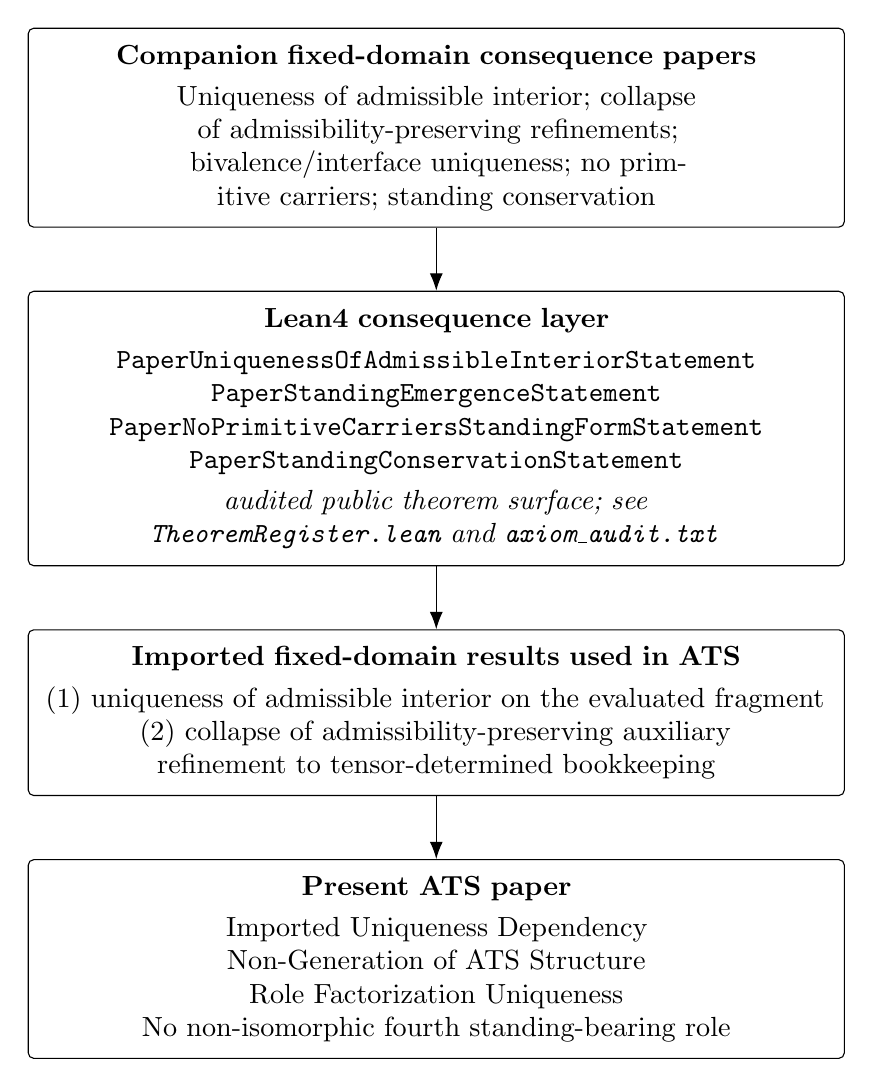
\begin{tikzpicture}[
  node distance=8mm and 12mm,
  box/.style={draw, rounded corners=2pt, align=center, text width=0.82\textwidth, inner sep=6pt},
  smallbox/.style={draw, rounded corners=2pt, align=left, text width=0.82\textwidth, inner sep=6pt},
  >={Latex[length=2.2mm]}
]
\node[box] (papers) {\textbf{Companion fixed-domain consequence papers}\\[0.3em]
Uniqueness of admissible interior; collapse of admissibility-preserving refinements;\\
bivalence/interface uniqueness; no primitive carriers; standing conservation};

\node[box, below=of papers] (lean) {\textbf{Lean4 consequence layer}\\[0.3em]
\texttt{PaperUniquenessOfAdmissibleInteriorStatement}\\
\texttt{PaperStandingEmergenceStatement}\\
\texttt{PaperNoPrimitiveCarriersStandingFormStatement}\\
\texttt{PaperStandingConservationStatement}\\[0.3em]
\textit{audited public theorem surface; see \texttt{TheoremRegister.lean} and \texttt{axiom\_audit.txt}}};

\node[box, below=of lean] (imports) {\textbf{Imported fixed-domain results used in ATS}\\[0.3em]
(1) uniqueness of admissible interior on the evaluated fragment\\
(2) collapse of admissibility-preserving auxiliary refinement to tensor-determined bookkeeping};

\node[box, below=of imports] (ats) {\textbf{Present ATS paper}\\[0.3em]
Imported Uniqueness Dependency\\
Non-Generation of ATS Structure\\
Role Factorization Uniqueness\\
No non-isomorphic fourth standing-bearing role};

\draw[->] (papers) -- (lean);
\draw[->] (lean) -- (imports);
\draw[->] (imports) -- (ats);
\end{tikzpicture}
\end{center}

\subsection*{Dependency table}

{\footnotesize
\renewcommand{\arraystretch}{1.15}
\begin{longtable}{@{}p{0.25\textwidth}p{0.27\textwidth}p{0.26\textwidth}p{0.16\textwidth}@{}}
\toprule
\textbf{Claim used in ATS} & \textbf{Imported content required} & \textbf{Lean4 witness / audited surface} & \textbf{Role in ATS}\\
\midrule
\endfirsthead
\toprule
\textbf{Claim used in ATS} & \textbf{Imported content required} & \textbf{Lean4 witness / audited surface} & \textbf{Role in ATS}\\
\midrule
\endhead
Uniqueness of the positive standing-bearing region & Fixed-domain uniqueness of admissible interior on the evaluated fragment & \texttt{PaperUniquenessOfAdmissibleInteriorStatement} & Fixes the extensional positive region used by the role decomposition\\
Collapse of stricter same-scope standing-bearing refinement beneath tensor content & Collapse of admissibility-preserving auxiliary refinements to bookkeeping / no primitive carrier form & \texttt{PaperNoPrimitiveCarriersStandingFormStatement} & Blocks nontrivial auxiliary standing layers and supports tensor-role uniqueness\\
Bivalence of standing-bearing classification & Fixed-domain standing/emergence and interface-level collapse to admissible vs.\ inadmissible & \texttt{PaperStandingEmergenceStatement} & Excludes intermediate standing-bearing role values at fixed scope\\
No creation, amplification, transfer, or repair of standing & Standing conservation / no-generator / no-carrier / no-repair consequence layer & \texttt{PaperStandingConservationStatement} & Forces anchor/tensor/skin to exhaust standing-bearing work\\
Non-generation of ATS structure & Imported fixed-domain consequence layer plus local ATS role analysis & Imported; corollary-level use in present paper & Shows ATS adds no new admissibility criterion, invariant, or operator\\
Role Factorization Uniqueness & Uniqueness of admissible interior + collapse of admissibility-preserving refinements + local role partition argument & Corollary assembled from imported Lean-backed results & Yields uniqueness of the ATS role decomposition up to isomorphism\\
\bottomrule
\end{longtable}
}

\subsection*{How to read the dependency}
The order is strict:
\begin{enumerate}[leftmargin=*]
    \item the companion fixed-domain consequence papers establish the relevant uniqueness and collapse results at theorem level;
    \item the Lean4 consequence layer witnesses those results on the audited public theorem surface;
    \item the present paper imports those results and proves the ATS decomposition as a corollary-level role factorization on that fixed substrate.
\end{enumerate}
Accordingly, the present paper should not be read as claiming that the fixed-domain uniqueness burden is first discharged here. What is first discharged here is the role-theoretic consequence: once admissible interior is unique and admissibility-preserving refinements have collapsed, the remaining standing-bearing work factors canonically into anchors, tensors, and skin.

\subsection*{Negative clarification for referees}
This appendix records three limits on the proof burden:
\begin{enumerate}[leftmargin=*]
    \item the present paper does \emph{not} claim that the ATS decomposition is independently foundational;
    \item the Lean4 formalization does \emph{not} need to encode the present ATS proposition as a new primitive theorem in order for the present result to be supported;
    \item if a referee wishes to challenge ATS uniqueness, the correct target is the companion uniqueness/collapse results or their Lean witnesses, not an alleged gap in the local ATS factorization argument.
\end{enumerate}

\subsection*{Minimal referee checklist}
A referee who wishes to audit the dependency structure need only verify:
\begin{enumerate}[leftmargin=*]
    \item that the companion consequence layer proves uniqueness of admissible interior and collapse of admissibility-preserving refinement at fixed scope;
    \item that the corresponding public Lean declarations are present and audited;
    \item that the present proposition uses those results only as imported fixed-domain consequences; and
    \item that the local ATS argument adds no new admissibility-bearing structure and only factors standing-bearing work into preconditions, invariant content, and representational surplus.
\end{enumerate}
Once those four checks are satisfied, the uniqueness and non-generation posture of the present paper is fully accounted for.


\end{document}